\hypertarget{RatingCurveBoundaryFormat}{}
\subsection{Hydro\_boundary\_rating\_curve.txt}
\index{Boundary}
\subsubsection{Purpose}
This file is made to prescribe the rating-curve type boundary conditions for hydrodynamics (number, type and values). These conditions come in addition to time series boundary condition.
%
\subsubsection{Input file format}
 \begin{tabular}{p{6cm} | p{9cm}}
    \hline
    Field(s) & Comment(s) \\
    \hline  \hline
    \texttt{\textbf{\#Comment   } } & Comment line, could be changed but not removed \\ \hline
    \texttt{\begin{tabular}{l}Description of the rating curve \\ bc\_code	-3 \\ type	interp \\	z0	0.4 \\\emph{LINE 5}\\ \emph{LINE 6}\end{tabular}
} & each rating curve $\Rightarrow$ 1 block of 6 lines.
    \begin{itemize}
    \item Line 1 : Comment line for the rating curve description, could be changed but not removed
		\item Line 2 : keyword \emph{bc\_code}: code of the boundary corresponding to the code assigned by the converter (see section \ref{sec:bc_file_format})
    \item Line 3 : keyword \emph{type}: type of the rating curve (allowed types, see below)
    \item Line 4 : keyword \emph{z0}: minimal elevation of the rating curve \emph{i.e.} if the water level within the cell is below than $z_0$ then the discharge is nil.
    \item Line 5 and Line 6 : depend of the type of rating curve
    \end{itemize} \\ \hline
	\end{tabular}  
\\
~\\ 
\paragraph{allowed types of rating curves}
\begin{description}
\item [interp] unit discharge is interpolated based on the water level $z$ within the cell using a curve $\left(z_{val}; q_{val}\right)$. If $z \le z_0$, the discharge is nil and if $z > \max\left(z_{val,i}\right)$, the unit-discharge is interpolated linearly based on the two last used-defined values (see figure below). The user has to define $\left(h_{val}; q_{val}\right)$ on line 5 and line 6 with $z_{val} = z_0 + h_{val}$.


 \begin{tabular}{p{5cm} | p{8.5cm}}

    \hline
    Field(s) & Comment(s) \\
    \hline  \hline
    \texttt{h\_val	0.00	0.50	1.00	1.50} & \begin{itemize}\item Line 5 : keyword \emph{h\_val} followed by a list of (positive and increasing) values of $h$. \end{itemize} \\
		\texttt{q\_val	0.00	0.07	0.20	0.37} & \begin{itemize}\item Line 6 : keyword \emph{q\_val} followed by a list of (positive) values of $q$. The lists $h_{val}$ and $q_{val}$ should contains the same number of values. By convention, the discharge is leaving the domain at a rating curve (thus negative) but the value are defined positively (the minus sign is added within the program). \end{itemize} \\
		\end{tabular}
		\\
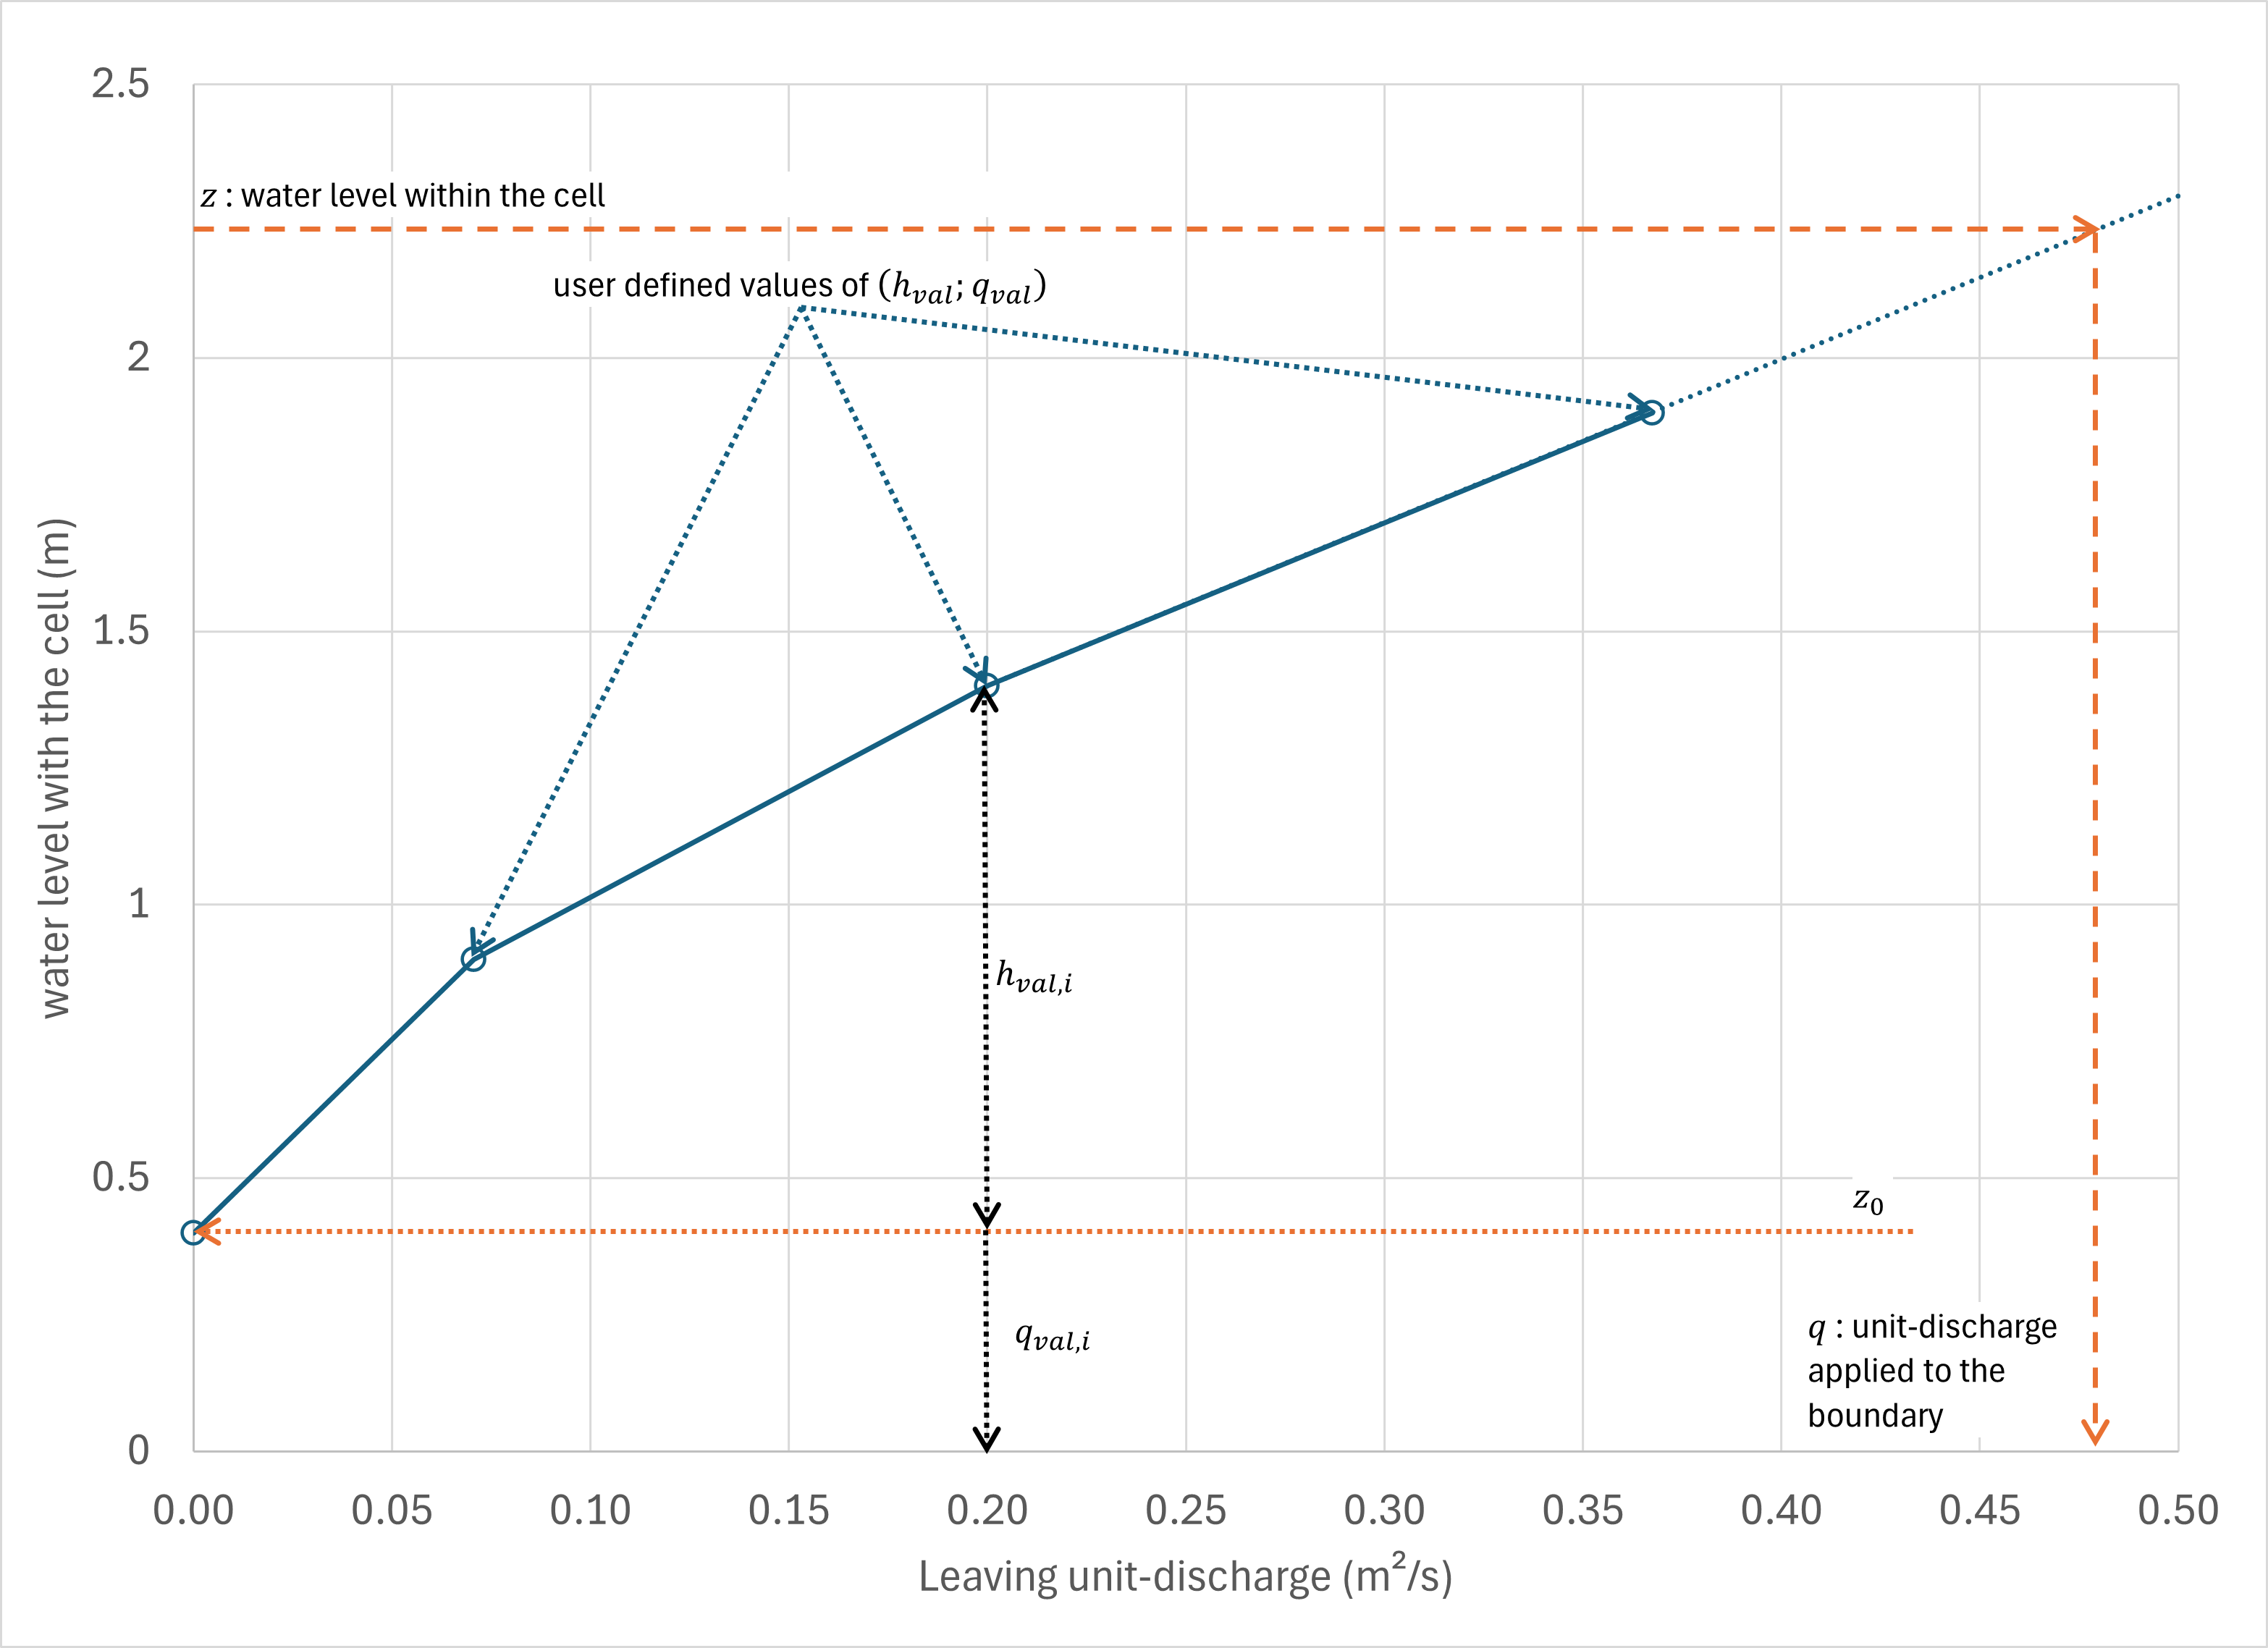
\includegraphics[width=0.7\columnwidth]{user/inputFile/RatingCurve.png}
		
\item [powerlaw] unit discharge is computed based on a powerlaw equation based on the water level $z$ within the cell:
\begin{subequations}\begin{eqnarray}
q = 0 & \texttt{if }  z < z_0 \\
q = a \left(z - z_0\right) ^ b & \texttt{otherwise}
\end{eqnarray}\end{subequations}

The user has to define the values of $a$ and $b$ on line 5 and line 6.


 \begin{tabular}{p{5cm} | p{8.5cm}}

    \hline
    Field(s) & Comment(s) \\
    \hline  \hline
    \texttt{a	0.20} & \begin{itemize}\item Line 5 : keyword \emph{a} followed by a positive number. By convention, the discharge is leaving the domain at a rating curve (thus negative) but the value of $a$ is defined positively (the minus sign is added within the program).\end{itemize} \\
		\texttt{b	1.5} & \begin{itemize}\item Line 6 : keyword \emph{b} followed by a non-nil number.  \end{itemize} \\
\end{tabular}
To avoid computational problems, the absolute value of $a$ and $b$ have to be greater than the program precision (defined to $10^{-16}$).
\end{description}   


		
%    
\subsubsection{Sample files}
\paragraph*{Example \#1}
Here, three rating curves are defined (with codes -2, -5 and -4). Defining three rating curve does not prevail that they will be used during the computation. If the bc\_code -5 has not be defined in the converter step (see section \ref{sec:bc_file_format}), the corresponding rating curve will be ignored.
\begin{verbatim}
\# each rating curve = 1 commented line (# or =) using followed by 5 lines containing the data (1st line is Always skipped)
\# 1st rating curve
bc_code	-2
type	interp
z0	0.4
h_val	0.00	0.25	0.50	0.75	1.00	1.25	1.50	1.75
q_val	0.00	0.125	0.354	0.650	1.000	1.398	1.837	2.315
\# 2nd rating curve
bc_code	-5
type	powerlaw
z0	0.4
a	0.44
b	2.50
\# 3rd rating curve
bc_code	-4
type	interp
z0	0.4
h_val	0.00	0.25	0.50
q_val	0.000	0.0125	0.0354
\end{verbatim}
